\documentclass[8pt,a4paper]{article}
\usepackage{graphicx}
\usepackage{amsmath}
\usepackage{amsfonts}
\usepackage{amssymb,amsthm}
\usepackage{array}
\usepackage[spanish, activeacute]{babel} %Definir idioma español
\usepackage[utf8]{inputenc} 

\voffset 0 cm \hoffset 0 cm \addtolength{\textwidth}{0cm}
\addtolength{\textheight}{0cm}\addtolength{\leftmargin}{0cm}

\begin{document}
%style file for ESANN manuscripts
\title{Procesamiento de texto manuscrito usando conjuntos de clasificadores}

%***********************************************************************
% AUTHORS INFORMATION AREA
%***********************************************************************
\author{
Emilio Samuel Aced Fuentes \\
Roberto Alcober Couso \\
Arturo Bl\'azquez P\'erez \\
Nicol\'as Trejo Moya \\
}
%***********************************************************************
% END OF AUTHORS INFORMATION AREA
%***********************************************************************

\maketitle

\section{Introducci\'on}
En este proyecto vamos a clasificar im\'agenes de letras manuscritas intentando predecir de forma correcta el s\'imbolo que representan.
Utilizaremos varios algoritmos de clasificaci\'on y los compararemos para encontrar los mejores resultados posibles, viendo diferencias de tiempos y  tasa de acierto.


\section{An\'alisis de los datos}
En el dataset provisto, est\'an representadaslas 10 primeras letras del alfabeto(A-J), por tanto 10 clases las cuales hemos etiquetado en nuestra base de datos etiquetadas de 0 a 10 respectivamente.
Las imagenes nos vienen en un tamaño de $206\times150$ en escala de grises.


\begin{figure}[htbp]
    \includegraphics[width=0.8\textwidth,natwidth=206,natheight=150]{./sin_procesar/l00000_A.png}
    \caption{Ejemplo de una A}
\end{figure}




Como podemos observar las imagenes contienen ruido, el cual podría dificultar la tarea de clasificación gravemente.Este problema lo hemos solucionado sometiendo a la imagen a diferentes tratamientos.

\subsection{Tratamientos}

Para todos los experimentos de este proyecto hemos umbralizado la imágen mediante otsu y posteriormente hemos realizado un filtro de mediana con un kernel cuadrado de tamaño 3.
Esto nos ha dado el siguiente resultado:
\begin{figure}[htbp]
    \includegraphics[width=0.8\textwidth,natwidth=206,natheight=150]{./procesado/l00000_A.png}
    \caption{Ejemplo de una A tratada}
\end{figure}

A continuación explicaremos los tratamientos que le hemos aplicado a las imágenes para reducir la complejidad del problema

\subsection{Atributos}
Teniendo en cuenta que las imágenes son matrices $206\times150$ lo cual nos da un total de 30900 atributos, lo cual es una cantidad de atributos desorbitada, por ese motivo hemos decidido ver como afecta reducir la dimensión.
Las principales modificaciones que realizaremos a las imagenes para reducir su dimensionalidad son las siguientes:

\paragraph{Eliminar filas y columnas poco importantes}


Esto lo realizaremos mediante la selección de un umbral, con el cual consideraremos que las filas y columnas que tengan una cantidad menor de zona pintada que el umbral especificado no son de relevancia y por tanto las despreciaremos del problema

\begin{figure}[htbp]
    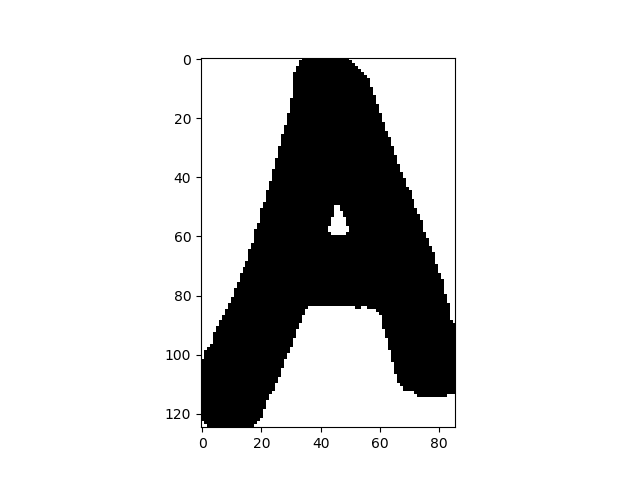
\includegraphics[width=0.8\textwidth,natwidth=206,natheight=150]{./Arecortada.png}
    \caption{Ejemplo de una A recortada}
\end{figure}

\paragraph{Redimensionar la imágen interpolando}

Con el fin de evitar el aliasing (meter bordes que no existian al reducir una imágen) hemos redimensionado la imágen siempre aplicando un kernel gausiano previamente.

A continuacion mostraremos distintos valores de los tamaños de las imágenes que compararemos en nuestro estudio:

\begin{figure}[htbp]
    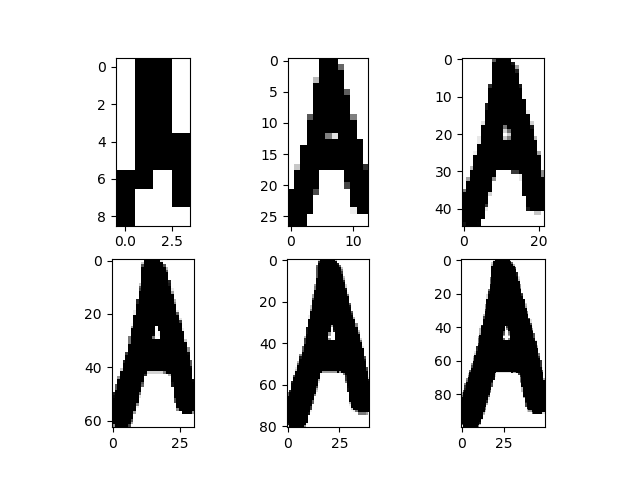
\includegraphics[width=0.8\textwidth,natwidth=206,natheight=150]{./A_Variando_Tam.png}
    \caption{Varios tamaños de una A que usaremos}
\end{figure}


\section{Modelos}

Usaremos los siguientes clasificadores en este trabajo:
\begin{enumerate}
\item Random Forest
\item SVC
\item KNN
\end{enumerate}
en los cuales variaremos los tamaños de las imágenes y compararemos tiempos y tasa de aciertos para poder decidirnos por uno.

Para todos ellos destinaremos la mitad de los datos para train y la otra mitad para test.

\subsection{Random Forest}



\end{document}
